% Written by
% Omur Ugur
% Email: ougur@metu.edu.tr
%
% can be any class (with options) hopefully
% a4paper and 12pt options are not mandatory, but preferred 
\documentclass[a4paper, 12pt]{article} % for a simple paper
%\documentclass[a4paper, 12pt]{report} % for a term project

% Language Specific (generally not neede):
%\usepackage[T1]{fontenc} 
%\usepackage[utf8]{inputenc}
% it is important that you load this package: iamPaperStyle.sty
\usepackage{iamPaperStyle} %includes also graphicx.sty and xcolor.sty

% any other styles you need
% not mandatory, but helful 
\usepackage{graphicx} % although loaded by iamPaperStyle.sty
\usepackage{amsmath, amssymb, amsthm} % others
\usepackage{hyperref} % other

% you may use a bit larger area on an a4paper in the document by
\usepackage{a4wide} % not necessary but generally useful


% now you may begin
\begin{document}

\studentName{Mutlu Çelik}
\advisorName{Prof.~Dr.~Omur Ugur}
% Your Department: 
% Scientific Computing, 
% Financial Mathematics, 
% Cryptography, or 
% Actuarial Sciences
\departmentName{Scientific Computing}
% Type of the Document:
% Preprint # may not work as expected (to-do)
% Qualification in PhD
% Report for Thesis Monitoring Committee
% Term Project
% Draft of a Manuscript
\paperType{Term Report}


\paperTitle{%
	One Dimensional Thermal Analysis Model for Charring Ablative Materials
}

\paperAuthor{%
  \"{O}. U\u{g}ur\footnote{%
    Middle East Technical University, Institute of Applied
    Mathematics, 06800 \c{C}ankaya, Ankara, Turkey. \hfill
  \emph{E-Mail}: \texttt{ougur@metu.edu.tr}},
	% possibly your advisor and co-advisor
  M. Celik\footnote{ Middle East Technical University, Institute of Applied
    Mathematics, 06800 \c{C}ankaya, Ankara, Turkey. \hfill
  \emph{E-Mail}: \texttt{mutlu.celik@metu.edu.tr}},
}

% abstract should not be large to fit in the title/front page
\paperAbstract{%
 This paper presents a one-dimensional model for the analysis of the charring ablative materials used in spacecraft 
thermal protection systems. The numerical method is based on an implicit finite difference formulation of the governing equations 
written for a system of mobile coordinates that accounts for the possible presence of surface recession. The maximum allowable 
operating temperature for the adhesive layer of the junction between the heat shield and the substructure is used as a design 
parameter for determining the minimum heat shield thickness. A case study on the re-entry of the Stardust capsule is presented. 
The model proposed as a useful dimensioning tool for the preliminary design phase of the heat shields of spacecraft entering 
the atmosphere. The model was validated through a survey of the literature related to the dimensioning of thermal shields, but 
based on numeric programs of highly representative industrial standards.
}

\paperKeywords{%
  Thermal protection system, Ablative materials, Thermal analysis
}

\paperDate{July 2021}

 % edit this file or see the lines below
%%%%%%%%%%%%%%%%%%%%%%%%%%%%%%%%%%%%%%%%%%%%%%%%%%%%%%%%%%%%%%%%%%%%%
% you may also use the predefined macros also here to over-write the
% info in the included file newPreprintDetails.tex

% \studentName{Ömür Uğur}
% \advisorName{Prof.~Dr.~Hamdullah Yücel}
% \departmentName{Scientific Computing}
% \paperType{Draft of a Manuscript}
% \paperTitle{This is the Title}
% \paperAuthor{\"{O}. U\u{g}ur, A. Mehmet}
% \paperAbstract{This is the Abstract} 
% \paperKeywords{Keyword 1, no keyword, illegalWord}
% \paperDate{April 2013} 

%%% mandatory:
\makePaperCoverPage
% for printing (and submitting) uncomment below (to have a sigle title page)
%\blankpage
%%%%%%%%%%%%%%%%%%%%%%%%%%%%%%%%%%%%%%%%%%%%%%%%%%%%%%%%%%%%%%%%%%%%%


%%%%%%%%%%%%%%%%%%%%%%%%%%%%%%%%%%%%%%%%%%
% The rest of the manuscript is trivial...
%%%%%%%%%%%%%%%%%%%%%%%%%%%%%%%%%%%%%%%%%%
% Hoever, try not to use commands like
% \title, \author, \date, \maketitle or \tableofcontents
% unless you need them of course: 
% you might need a title and a table of contents
% at the begining sometimes
%\title{Title of the Manuscript}
%\author{Author Name Surname}
%\date{\today}
%\maketitle

% if necessary (suggested in a simple paper submitted to IAM}
\makeTitle % don't use this if this is a term project
\tableofcontents % will be a separate page in case of term project


%%%%%%%%%%%%%%%%%%%%%%%%%%%
% CONTENT OF THE MANUSCRIPT
%%%%%%%%%%%%%%%%%%%%%%%%%%%

% instead of typing here inside this document
% we suggest you to include or input a
% separate document of yours:
% \input{yourdocname}

% For Reports un comment \chapter{}
%\chapter{In case of a Report Chapter is needed}
%		\label{chap:ReportIntro}
\newpage
\section{Introduction} \label{sec:first_intro}
Thermal management is an important part of high speed vehicles like aircrafts, space shuttles and missiles. For high aerothermal loads, many different thermal protection systems(TPS) are developed. One easy and efficient way is to use ablative TPS materials to dissipate high entering heat flux which is widely used for aerospace systems as heat shield(covering main structure). Therefore, modelling of ablation phenomenon becomes very important while deciding the feasibility of  design from thermal point of view. Ablation simply means degradation or removing of a material surface due to chemical reactions, erosion or vaporization and there are mainly two classes of ablative materials: "charring" and "non-charring". Ablative material called as non-charring if the material does not have any chemical reaction during removal process( like a simple change of state), it is called as charred if high heat causes a chemical reaction inside the material which leads to leakage of pyrolysis gases. Mainly, charring ablative materials contain resin which decomposes and generates gas when heated adequately, this is an endothermic reaction which is called as "pyrolysis". This reaction starts from the upper part of material where thermal loads are present and when this reaction is done remaining material called as "char" or "charred material". If material does not reach necessary temperature for pyrolysis reaction, it is called as "virgin ablative material". The outflow gases ,which are produced during pyrolysis reactions, pass through porous structure of charred ablative material and behaves like a barrier against aero-thermal heating(convective heating, radiative heating), this is another thermal protection effect of ablative materials. Lastly, during whole this process surface recession occurs due to mechanical erosion on charred part which causes a consistent decrease of material thickness. This general structure described is shown on Figure ~\ref{fig:char_model} as shematic\cite{mazz}. \newline
\begin{figure}[h!]
  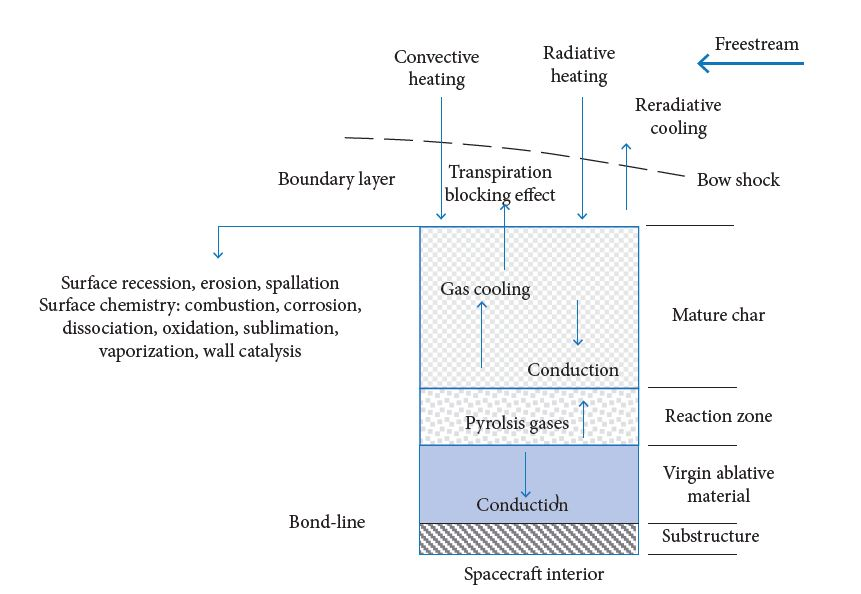
\includegraphics[width=\linewidth]{char_model.jpg}
  \caption{Shematic of charring ablative thermal protection system}
  \label{fig:char_model}
\end{figure}
Until 1950s no research was done about modeling or application of ablation phenomenon because there was no need for such a thermal protection system. Firstly space engineers and researchers began thinking about how to return from space, especially from thermal point of view since atmospheric reentry is an important thermal challenge due to high heat loads, . To overcome this challenge many different vehicle designs are tested through wind tunnels but just changing the design of the vehicle were not enough. Even they could cope with thermal loads weight increase became problem for trajectories due to using of high density metals such as copper as heat sink structure or using of very thick metal bodies then first considerations have started about ablative materials\cite{bian}. After committed assesments and analysis by researchers, using of ablative thermal protection system for atmospheric reentry became an important and logical choice due to its low density and high heat absorption properties. At this point, modelling of ablation became important of scientists and engineers. In 1965, a significant Nasa Technical Note is published by Donald M. Curry which gives a detailed mathematical model for charring ablation thermal protection system\cite{cury}. He used 1D implicit finite difference method to formulate differential equations and developed a FORTRAN IV code to make necessary calculations. That paper also showed the verification of the model by experimental results. These mathematical model and its verification enable engineers to calculate minimum thickness required for the missionans this leads to usign of ablative TPS for first successful controlled reentry mission of NASA\cite{Gemini}(Gemini 6A, Figure Figure ~\ref{fig:gemini}) which is a manned reentry mission and then it is used şb many space missions till today. It is still a commonly used TPS for atmospheric re-entry missions.\newline

\begin{figure}[h!]
  \centering
  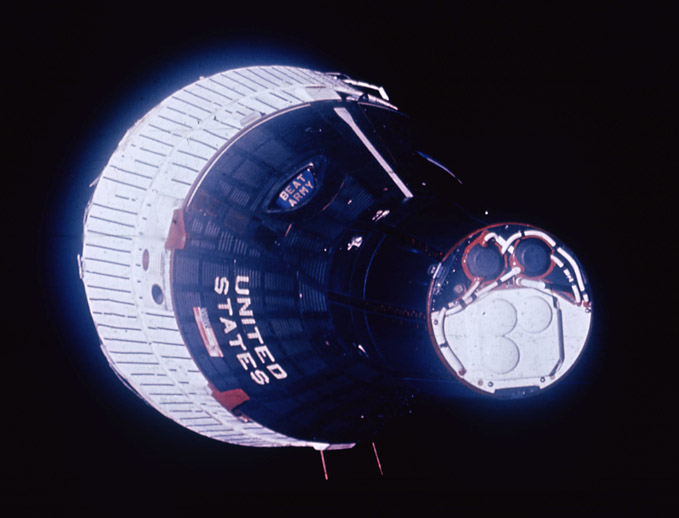
\includegraphics[width=0.8 \linewidth]{gemini_6.jpg}
  \caption{Gemini 6A spacecraft, black side is charring ablative TPS(painted)}
  \label{fig:gemini}
\end{figure}



\section{TheAblative Thermophysical Model}
Mathematical model presented here is also a 1D implicit model and specific for charring ablative materials. This model is suggested to be used in conceptual development phase since it gives faster result comparing to other detailed models. Here instead of using whole trajectory of a space vehicle, just stagnation point, where heat flux is maximum, is enough to find necessary results for conceptual development case. As it is described in section 1, the aim is to find minimum thickness required that keeps the body structure below maximum operating temperature.
\subsection{Assumptions}
Before explaining the governing equation of the model the assumptions made for ablation physics are described in this section. Seven main assumptions are explained below.

\begin{enumerate}
 \item In fact it is not easy to know exactly where decomposition of virgin state material to char occurs but in this model it is assumed in a certain area which is called as reaction zone. 
 \item There are two important temperature values defining the reaction zone: $T_{abl}$, temperature where pyrolysis reactions start; $T_{char}$, temperature where fully charring occurs. These temperature values are found by assessing the thermogravimetric experiments. One sample graph is given in Figure ~\ref{fig:tga}. As it seen, these temperature points are estimated by looking at the behaviour of the curvature.
\begin{figure}[h!]
  \centering
  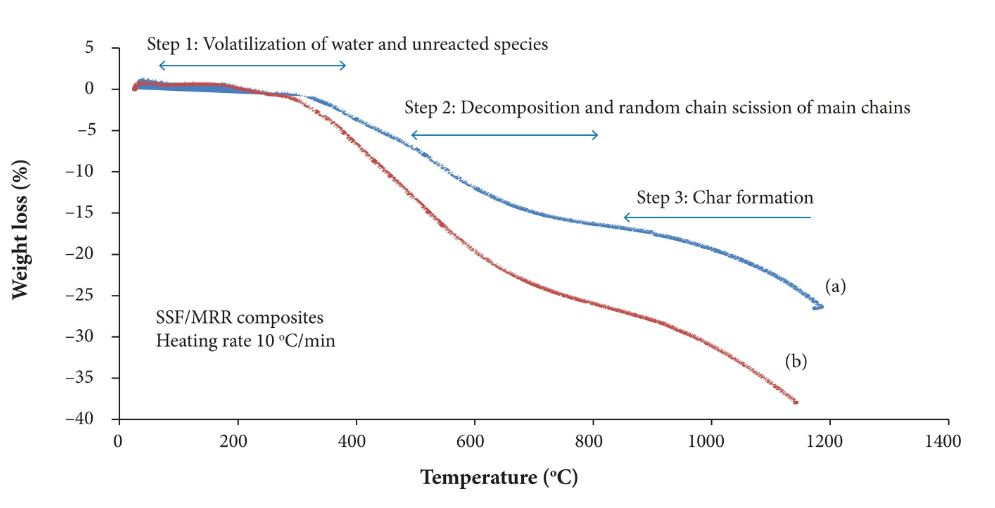
\includegraphics[width= \linewidth]{tga.jpg}
  \caption{Thermogravimetric experiment data for short silica fiber, reinforced modified resole resin composites(SSF/MRR) under (a) nitrogen and (b) air flow. \cite{elw}}
  \label{fig:tga}
\end{figure}
\item Pressure loss during upward flow of the gases generated in the reaction zone to upper parts is neglected. (It is assumed that gas instantenously passes to upper layers.)
\item Effects of thermal stress is neglected.
\item There is a local thermal equilibrium between the char zone and gases.
\item Rather than the reactions described in the model, there is no chemical reaction occurs betweeb gases and environment.
\item Thermal effects of internal part of spacecraft is neglected.

\end{enumerate}


\subsection{Governing Equations}
Equations to estimate the physics of ablation are explained in this section. Main equations are: The internal energy equation which describes the accumulation rate of thermal energy, internal decomposition equation that the decomposition rate due to pyrolysis reactions, surface energy balance equation to calculate net total heat flux at the surface, surface recession that calculates the total char removal from surface.
\subsubsection{The Internal Energy Balance Equation}

\begin{eqnarray} \label{en_eq}
\rho c_p \frac{\partial T}{\partial t}\biggr|_x=\frac{\partial}{\partial x}(k\frac{\partial T}{\partial x}-\dot{q}_R)\biggr|_t+(H_d-\bar{h})\frac{\partial \rho}{\partial t}\biggr|_y+\dot{S} \rho c_p\frac{\partial T}{\partial x}\biggr|_t+\dot{m_g}\frac{\partial h_d}{\partial x}\biggr|_t
 %\psi_t  = i\psi_{xx} + i\gamma \vert \psi \vert^2\psi
\end{eqnarray}
In this equation $\rho$: Density$(kg/m^3$), $c_p$: Specific heat at constant temperature(J/(kg.K)), T: Temperature(K) , k: Thermal conductivity(W(m.K)), $\dot{q_R}$: Internal radiative heat flux($W/m^2$), $H_d$ : Pyrolysis enhalpy(J/kg), $\bar{h}$: Partial heat of charring(J/kg) given in Eq. , $\dot{S}$: Char recession rate(m/s)  $\dot{m}_g $: Pyrolysis gas mass flow rate($kg/m^2s$)), x: Mobile coordinate system(m) that is moving with the surface recession and y: Fixed coordinate system at the beginning of the analysis these two systems are coincident. \par
As it is described before this equation gives the accumulation rate of thermal energy. The terms of rightern side represents respectively conduction and internal radiation, energy consumption due to pyrolysis, convective rate caused by surface recession and caonvective rate due to pyrolysis gases. It is clearly seen some material dependent properties($c_p$, $\rho$ and $k$) are used while modelling internal energy balance. During ablation the state of the material is between char and virgin states because of that these material properties have to be considered with some approximations given below. Here $\tau$ is the mass fraction of the virgin material with respect to total weight given in Eq. \ref{tau}. Subscript 'v' refers to virgin state and 'c' refers to char state. The equation of specific heat ($c_p$) and thermal conductivity($k$) is given in Eq. \ref{cp} and Eq.\ref{k}. For density linear relation with respect to temperature is considered(it is commonly used equation for reaction zone).
\begin{eqnarray} \label{tau}
\tau=(1-\rho _c/\rho)/(1-\rho _c /\rho _v)
\end{eqnarray}
\begin{eqnarray} \label{cp}
c_p=\tau c_{pv}+(1-\tau)c_{pc}
\end{eqnarray}
\begin{eqnarray} \label{k}
k=\tau k_v+(1-\tau)k_c
\end{eqnarray}
\begin{eqnarray} \label{rho}
\rho=(\rho _v - \rho _c)\frac{T-T_{abl}}{T_{char}-T_{abl}}
\end{eqnarray}
\newline
Lastly, pyrolysis gas's enthalphy($h_d$) is depend on temperature and pressure but the partial heat of charring($\bar{h}$) can be defined  as in Eq. \ref{par_h}.
\begin{eqnarray} \label{par_h}
\bar{h}=\frac{\rho _vh_v - \rho _ch_c)}{\rho _v-\rho _c}
\end{eqnarray}


\subsubsection{The Internal Energy Balance Equation}
This equation used for pyrolysis decompostion part of energy equation. It is developed based on Arrhenius relationship by adopting the coefficients for complete plastic ablative composite.
\begin{eqnarray} \label{Arr}
 \frac{\partial \rho}{\partial t}=K(\frac{\rho - \rho _c}{\rho _v-\rho _c})^ne^{-B/T}
\end{eqnarray}

\subsubsection{Internal Mass Balance Equation }
This equation gives the mass flow rate of the pyrolysis gases. In this model it is approximated as equal to pyrolysis decomposition.
\begin{eqnarray} \label{m_g}
\frac{\partial \dot{m_g}}{\partial y} =\frac{\partial \rho}{\partial t}
\end{eqnarray}
\subsubsection{Surface Energy Balance Equation }
On the surface of the ablative material there is a high heat flux  due to convective,radiative heat transfer and thermochemical interactions. This equation gives the net total heat flux at the surface which is also boundary.
 \begin{eqnarray} \label{Arr}
\dot{Q}_{in}=\dot{q}_{c,blow}+\dot{q}_{rad}+\dot{q}_{comb}-F\sigma \epsilon (T_w^4-T_{\inf}^4)
\end{eqnarray}
Where $\dot{Q}_{in}$: Net total heat flux at the surface($W/m^2$), $\dot{q}_{c,blow}$: net hot wall convective heat flux($W/m^2$), $\dot{q}_{rad}$: Entering radiative heat flux ($W/m^2$), $\dot{q}_{comb}$: Combustion heat flux ($W/m^2$), F: View factor,$ \sigma$ : Stefan-Boltzmann constant ($W/m^2K^4$),$ \epsilon$ : Surface emissivity, $T_w$: Wall temperature(K), $T_{\inf}$: Free stream temperature(K) \newline
To be able to express the terms on the rightern side, equation of some coefficients should be declared(Eq. \ref{hw} - Eq. \ref{Ac}) . V is the velocity of spacecraft and $c_{patm}$ is the specific heat of atmosphere.

 \begin{eqnarray} \label{hw}
h_w=c_{patm}T_w
\end{eqnarray}
\begin{eqnarray} \label{h0}
h_0=c_{patm}T_{\inf}+\frac{V^2}{2}
\end{eqnarray}
\begin{eqnarray} \label{Ac}
A=\frac{h_0}{\dot{q}_{c,w}}(\alpha _c \dot{m_c} +\alpha _g \dot{m_g})
\end{eqnarray}
$\dot{q}_{c,w}$: Cold wall convective heat flux($W/m^2$), $\dot{m_c}$: Removal rate of char due to surface recession($kg/(m^2s)$), where the coefficients $\alpha_c$ and $\alpha_g$ are
used to consider the molecular weight of gases in the boundary layer from that of the injected pyrolysis gases. The coefficient $\alpha_c$ also takes into account the part of the char that is mechanically removed rather than sublimated. Eq. \ref{Ac} is needed to approximate blocking effect of pyrolysis gases in the boundary layer. Lastly, Eq. \ref{qcon} gives the hot wall convective heat flux which will help for calculating net hot wall convective heat flux.
\begin{eqnarray} \label{qcon}
\dot{q}_{con}=\dot{q}_{c,w}(1-\frac{h_w}{h_0})
\end{eqnarray}
\newline
Now, the equations of the rightern side can be expressed. If coefficient A is smaller than 2.25 ($A<2.25$) then Eq. \ref{qblow1} is used, otherwise($A\geq2.25$) Eq. \ref{qblow2} is used for net how wall convective heat flux calculation.
\begin{eqnarray} \label{qblow1}
\dot{q}_{c,blow}=(1-0.724A+0.13A^2)\dot{q}_{con}
\end{eqnarray}
\begin{eqnarray} \label{qblow2}
\dot{q}_{c,blow}=0.04\dot{q}_{con}
\end{eqnarray}
\par
Secondly, heat flux effect of the combustion of the ablation products is expressed as in Eq. \ref{qcomb}.
\begin{eqnarray} \label{qcomb}
\dot{q}_{comb}=\dot{m_c}\Delta H_c
\end{eqnarray}

\subsubsection{Surface Recession }
Total recession due to surface material(char) removal can be easily defined as: 
\begin{eqnarray} \label{qcomb}
S=\int_{0}^{t} \dot{S}dt
\end{eqnarray}



\section{Shematic of The Ablative Thermal Model}
In introduction section the numerical approach of the paper is clearly indicated as 1D implicit difference formulation(backward time, centered space) which is used for governing equations explained in previous section. The advantage of this methodology is, especially in thermal field, by using parabolic partial differential equations, the resultant implicit scheme is unconditionally stable in both time and space. This approach is applied for the shematic given in Fig. ~\ref{fig:model} . Upper boundary is exposed to surface recession(moving to bottom) so it is called as free surface and recession is modeled continuously. Ablative material part (char,reaction zone, virgin ablative) splits into a predefined and fixed number of nodes with size $\Delta X$. Node number is increasing starting from upper node to bottom node. (In original paper there are three substructure but there is no need for extra two of them to express the main idea of the modelling) \newline
\begin{figure}[h!]
  \centering
  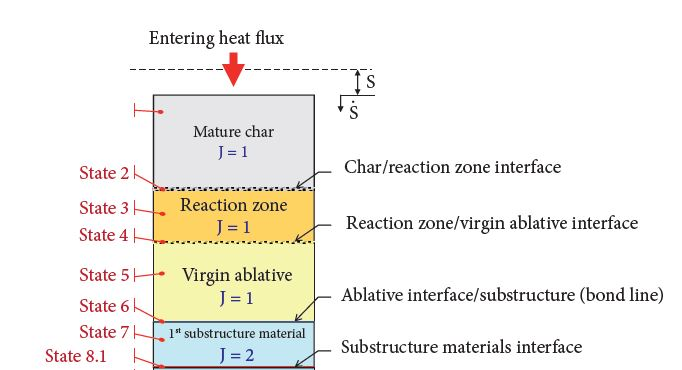
\includegraphics[width=0.8 \linewidth]{model.jpg}
  \caption{Schematic of the implemented model}
  \label{fig:model}
\end{figure}

The algorithm starts with estimation of ablative material thickness and determines the minimum thickness. The algorithm is basicly decreases the thickness values and stops when critical temperature values is reached(when temperature of the substructure material is higher than its operating temperature). While decreasing the thickness the secant method is used for smooth convergence(10-15 iterations. Newton method was also a good choice but author did not prefer it because of difficulty of estimating derivative. \par
After making necessary calculations and leave the unknown temperatures for nodes left-hand side and other values to right-hand side, Eq. \ref{nodal} is obtained. Consequently, we had a tridiagonal system of N nodes where our problem becomes as Eq .\ref{mat}. 
\begin{eqnarray} \label{nodal}
A_iT_{i-1}'+B_iT_{i}'+C_iT_{i+1}'=D_i
\end{eqnarray}
\begin{eqnarray} \label{mat}
 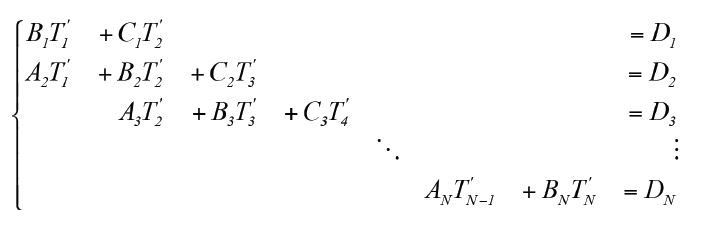
\includegraphics[width=0.8 \linewidth]{mat.jpg}
\end{eqnarray}

\subsection{Assumptions of Thermal Model}
While discretising the governing equations by finite differences, some key assumptions are done. In this section these assumptions, which are linearized radiation assumption, moving surface assumption and radiation between two parallel flat surfaces, will be explained.
\subsubsection{Linearized Radiation}
Radiation is calculated by using the fourth power of temperature and instead of taking fourth order of unknown temperature it is linearized and expression is adopted as Eq. \ref{rad}.
\begin{eqnarray} \label{rad}
(T_{i}')^4=(T_{i}+\Delta T)^4=T_{i}^4\biggr( 1+\frac{\Delta T}{T_{i}} \biggr)^4 \cong T_{i}^4\biggr(1+4\frac{\Delta T}{T_{i}} \biggr)=4T_{i}^3T_{i}'-3T_{i}^4
\end{eqnarray}
\subsubsection{Moving Surface(Surface Recession)}
Additional terms to the energy balance equations are used than by taking the derivative of thermal capacitive term(left-hand side term) surface recession rate is derived as seen in Eq. \ref{rec2}. NP means total number of nodes in the ablation material.

\begin{eqnarray} \label{rec1}
\frac{\partial}{\partial t} \biggr( \Delta X \rho c_pT \biggr) = \Delta X \rho c_p\frac{\partial T}{\partial t}+\rho c_pT\frac{\partial( \Delta X) }{\partial t}
\end{eqnarray} 
where
\begin{eqnarray} \label{rec2}
\frac{\partial( \Delta X) }{\partial t}=\frac{\partial}{\partial t}\biggr( \frac{S_{init}-S}{NP-1} \biggr)  = -\frac{\dot{S}}{NP-1}
\end{eqnarray}

\subsubsection{Radiation between two parallel flat surfaces}
While considering radiative relations the form factor is taken as 1($F_{12}=1$) and equivalent emissivity is calculated as shown in Eq. \ref{em}.
\begin{eqnarray} \label{em}
\epsilon _{eq}=\biggr( \frac{1}{\epsilon _1}+\frac{1}{\epsilon _2}-1\biggr)^{-1}
\end{eqnarray}

\subsection{Nodal Schemes}
Starting from the first node of surface nodal scheme for each part of the model is represented in Figure ~\ref{fig:node_1} -Figure ~\ref{fig:node_last} \cite{mazz}. Equations of each nodal scheme is also given in the figures. Red arrows mean energy addition and blue arrows mean removal of energy.
\begin{figure}[h!]
  \centering
  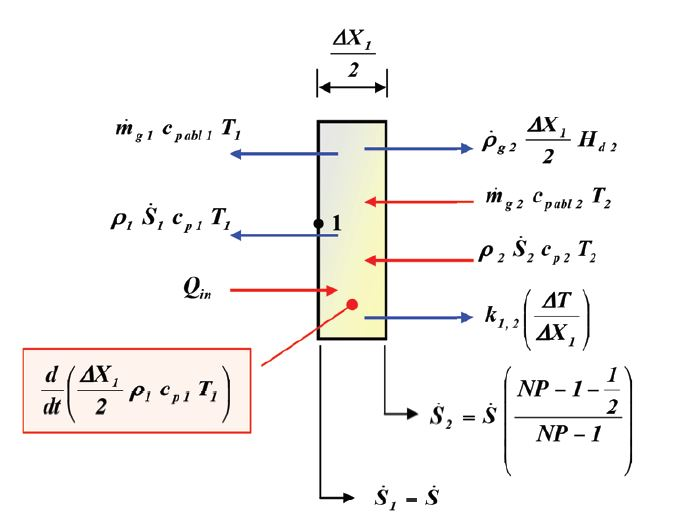
\includegraphics[width=0.6 \linewidth]{node_1.jpg}
  \caption{Nodal scheme of first node (upper surface)}
  \label{fig:node_1}
\end{figure}
\begin{figure}[h!]
  \centering
  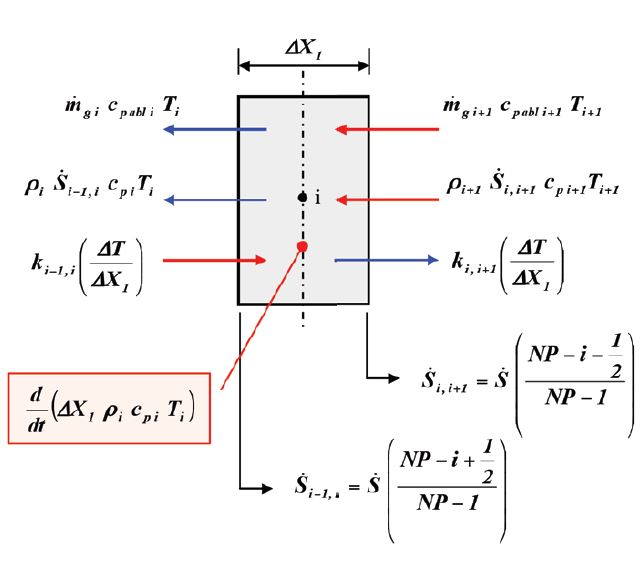
\includegraphics[width=0.6 \linewidth]{matur_nodal.jpg}
  \caption{Nodal scheme of state 1(matur char zone)}
  \label{fig:matur}
\end{figure}
\begin{figure}[h!]
  \centering
  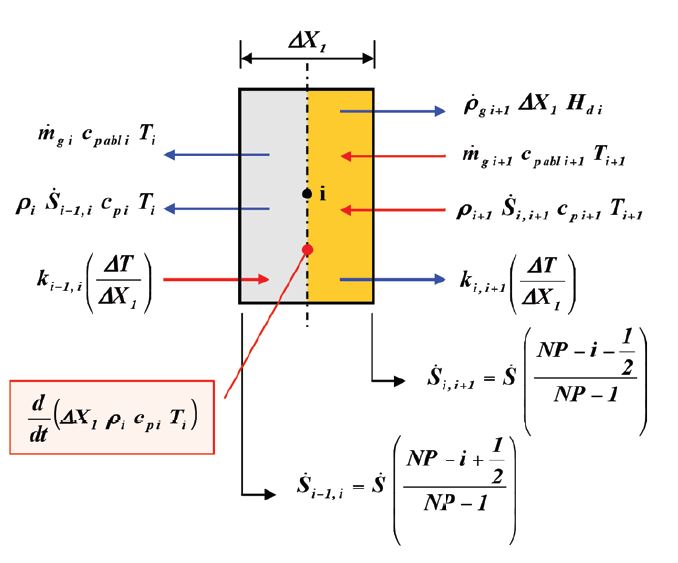
\includegraphics[width=0.7 \linewidth]{matur_react.jpg}
  \caption{Nodal scheme of state 2 (matur char-reaction zone interface)}
  \label{fig:mr}
\end{figure}
\begin{figure}[h!]
  \centering
  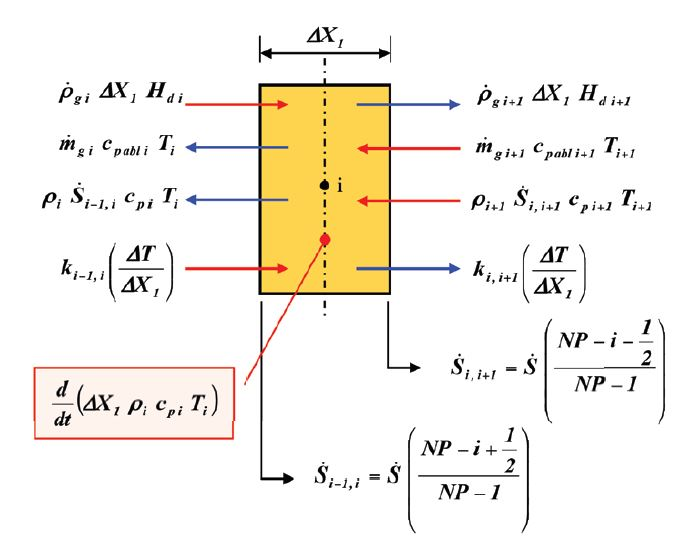
\includegraphics[width=0.7 \linewidth]{react_nodal.jpg}
  \caption{Nodal scheme of state 3(reaction zone)}
  \label{fig:react}
\end{figure}
\newpage
\begin{figure}[h!]
  \centering
  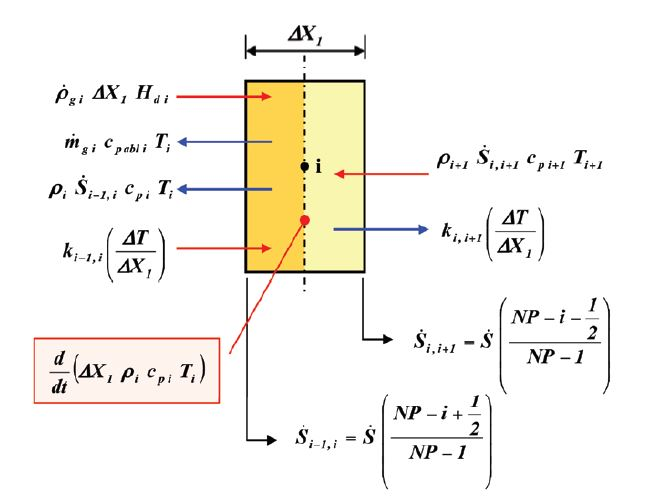
\includegraphics[width=0.75 \linewidth]{react_virgin.jpg}
  \caption{Nodal scheme of state 4(reaction zone-ablative virgin interface)}
  \label{fig:rv}
\end{figure}
\newpage
\begin{figure}[h!]
  \centering
  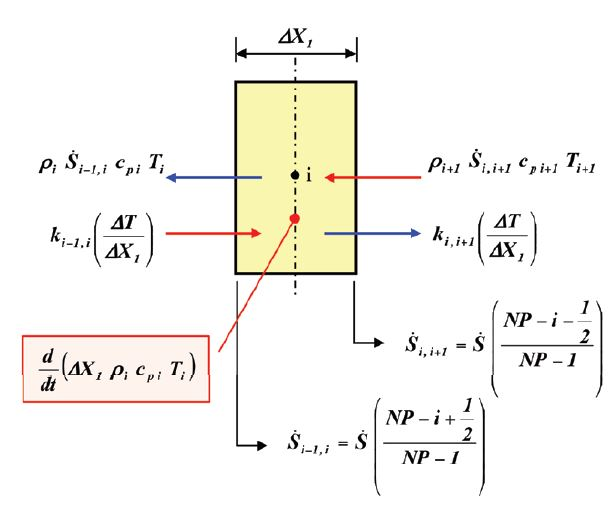
\includegraphics[width=0.75 \linewidth]{virgin.jpg}
  \caption{Nodal scheme of state 5(ablative virgin material)}
  \label{fig:vir}
\end{figure}
\begin{figure}[h!]
  \centering
  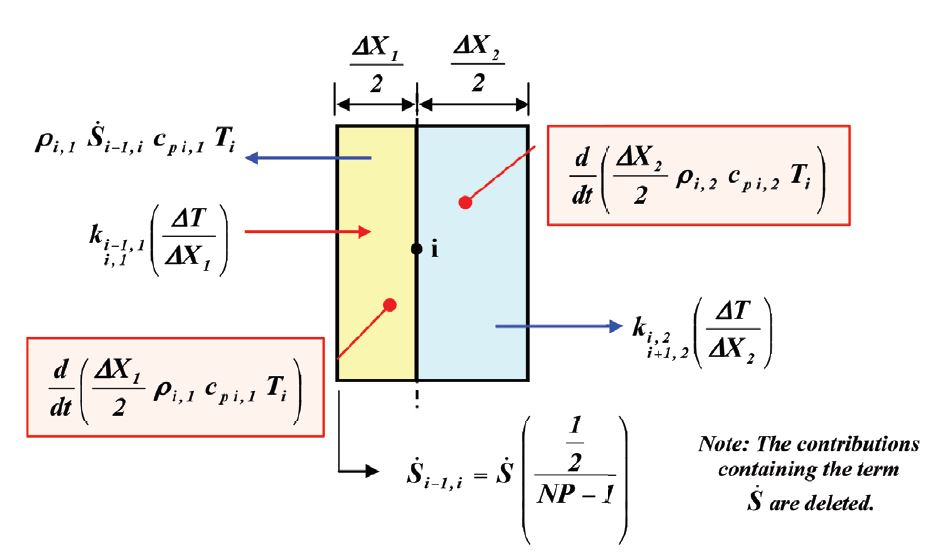
\includegraphics[width=0.82 \linewidth]{virgin_sub.jpg}
  \caption{Nodal scheme of state 6(ablative virgin interface-substructure material interface)}
  \label{fig:vs}
\end{figure}
\begin{figure}[h!]
\centering
  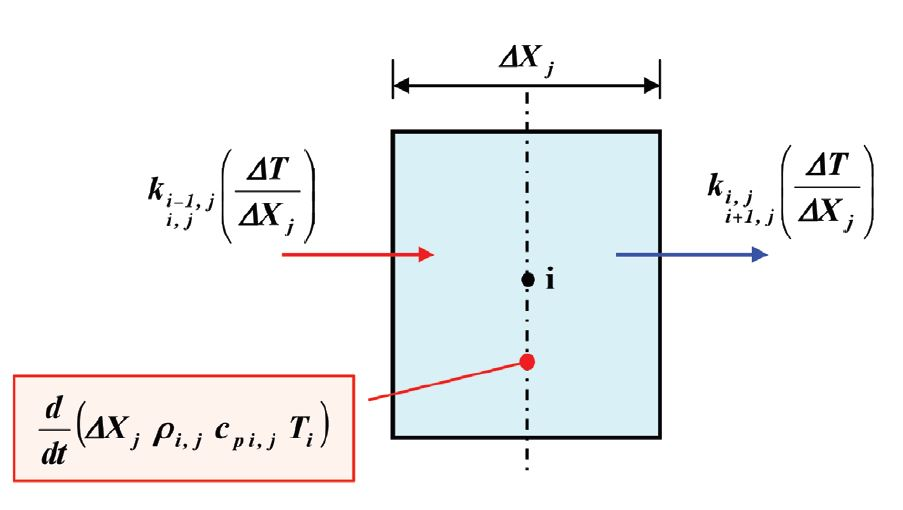
\includegraphics[width=0.6 \linewidth]{sub_nodal.jpg}
  \caption{Nodal scheme of state 7(substructure material)}
  \label{fig:sub}
\end{figure}
\begin{figure}[h!]
  \centering
  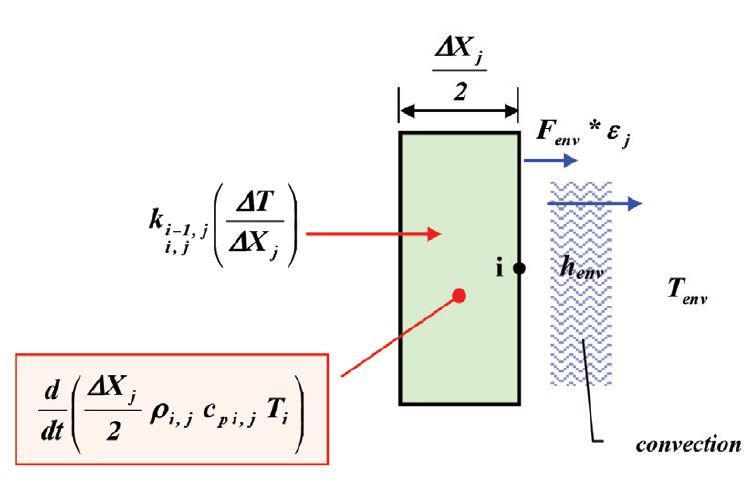
\includegraphics[width=0.6\linewidth]{node_last.jpg}
  \caption{Nodal scheme last node(substructure material with radiation and convection to cabin interior)}
  \label{fig:node_last}
\newpage
\end{figure}


\newpage
\section{Conclusion}
In this paper Mazzarachio's paper\cite{mazz} is summarized by explaining the one dimensional thermal analysis model for charring ablatives. This model is presented as a verified model and tried with Stardust return capsule as a case study. At the end of the paper Mazzarachio pointed the model's excellent agreement with similar literature data(especially with NASA's FIAT model). This result was very expected result because the numerical model Donald M. Curry proposed in 1965 \cite{cury} was nearly the same model(even the nodal scheme figures are same). As a further study of this research and ongoing researchs on this field, 2D model can be developed to see surface change of the TPS(since recession will be different depending on the thermal loads) and effects of this change to aerodynamic of the spacecraft can be investigated. Researches will continue for finite element models of this phenomena as well. 
\newpage


  









%%%%%%%%%%%%%%%%%%%%%%%%%%%%
% CONTENT ENDS HERE (almost)
%%%%%%%%%%%%%%%%%%%%%%%%%%%%



%%% The following way of Bibliography is not recommended

\begin{thebibliography}{99}
	\bibitem{mazz}  A. Mazzarachio.
 One-Dimensional Thermal Analysis Model for Charring Ablative Materials,
  J Aerospace Technology Management, V10,
  2018. 
%
	\bibitem{bian}  D. Bianchi. Modeling of Ablation Phenomena in Space Applications,
   Sapienza University of Rome, Department of Aerospace Engineering, 2007.
	%Academic Press Inc., Boston, MA, second edition, 1990.
\bibitem{elw}  I. Elwan, R. Jabra,M. H. Arafeh. Preparation and Ablation Performance of Lightweight Phenolic Composite Material under Oxyacetylene Torch Environment,
   Journal of Aerospace Technology and Management, 2018.
\bibitem{Gemini}  Grimwood, J. M., et al., Project Gemini technology and operations - A chronology, NASA, NASA SP-4002, Wash., DC, 1969.
\bibitem{cury}  D. M. Cury. An Analysis of Charring Ablation Thermal Protection System,
   Manned Spacecraft Center, NASA, 1965.
bibitem{laub} B. Laub. Ablative Thermal Protection an Overview. 55th Pacific Coast Regional and Basic Science Division Fall Meeting, Oakland, California, 2003.
\end{thebibliography}

%
% References in Bibtex format goes into below 
% indicated file with .bib extension
%\bibliography{myBiblio} filename: myBiblio.bib
% You can use full name of authors, 
% however most likely some of the Bibtex entries you will find, 
% will use abbreviated first names.
% If you don't want to correct each of them by hand, 
% you can use abbreviated style for all of the references
% \bibliographystyle{abbrv}
% However, IAM suggests to use
\bibliographystyle{iamBiblioStyle} % better than to use {plain or abbrv}

%%% APPENDIXES in case you need
%\appendix
%
% input your appendix
% If you are not using minted style, then comment the first appendix below
% otherwise uncomment.
%uncomment%  \input{appendix/app1} % includes minted package examples!
%\input{appendix/app2}


\end{document}

